\section{S3}
	\subsection{Context}
	The purpose of S3, as a data storage, is used to store all files, and these files include unformatted and uncleaned data and results integrated into analytics tool. S3 gains any types of data and format data from the user and then move them to other services in Amazon platform.
        
	\subsection{Composition}
	\textbf{Buckets:} bucket is a basic container used to store objects in S3.\cite{z1}
     
    \noindent \textbf{Objects:} Objects are the fundamental entities stored in S3, and it consists of object data and metadata. The role of metadata is to store set of name-value pairs that describe the object.\cite{z1}
        
	\noindent \textbf{Keys:} each object has the unique identifier and which is called “key”. In order to ensure uniqueness of each object, the combination of a bucket, key and version ID is used to identify each object in S3.\cite{z1}
    
	\subsection{Interaction}
    S3 need to upload data to analytics and send data to database, thus S3 will interact with the Data Pipeline, and then complete data transforming between different compute and storage services according to the application on data pipeline. On the other hand, the developer needs to program some functions for S3, thus S3 will interact with AWS Lambda. The role of AWS Lambda is to run code for all backed services on this platform.
    
	\subsection{Algorithm}
    The AWS SDK supports several programming languages to develop S3 by programming. The programming languages cover Java, .NET, Ruby, Python and PHP. On the other AWS SDK also provide many API for these programming languages. Take an instance with Java, the developer can utilize low-level API to implement create, update, and delete operations that apply to buckets and objects in S3.\cite{z2} 
   
\section{Amazon Kinesis}
	\subsection{Context}
    Parsing data like log file and streaming can ensure consistency and normalization of data which will be moved to database. Thus, the service Amazon Kinesis provides is complete the basic integrating and parsing for these data.
        
	\subsection{Composition}
    \textbf{Amazon Kinesis Firehose:} the key concept of Amazon Kinesis Firehose is to create a delivery stream and then the delivery stream is used to receive data from the user. Eventually, this delivery stream will be processed by Amazon Kinesis Analytics as the underlying entity of Firehose.\cite{z3}
    
    \noindent \textbf{Amazon Kinesis Analytics:} Amazon Kinesis Analytics support user uses a series of SQL statements to complete multiple operations for the stream. On the other hand, the developer can also develop own application to satisfy some special requirements.
     
    \noindent \textbf{Amazon Kinesis Streams:} the developer can create a stream through this composition.

	\subsection{Dependency}
    The service is not completely independent from others. The reason is it needs data from the external source such as S3, so the precondition of using this service is developer must have existing data.

	\subsection{Interaction}
    Amazon Kinesis must interact with other entities. There are two reasons. One is Amazon Kinesis needs to receive data from other services. Second reason is the results should be exported to other services after data parsed by Amazon Kinesis Analytics. 

	\subsection{Algorithm}
    The core concept of Amazon Kinesis Analytics is to create one or more applications for completing multiple tasks. The programming language is SQL in this composition, and it provides enough functions to solve some general problems.\\

	\noindent \textbf{Pre-processing streams:} The purpose of pre-processing streams is to normalize data and avoid errors appear before some applications do high-level processing because sometimes streaming source contains many kinds of extra conditions. For example, if the streaming source includes multiple record types, which means developers need to integrate all data from these two record types. In this condition, developers can create two additional in-application streams to store these two record types separately. And the filter the rows from the original source based on record type and insert them in the newly created streams using pumps.\cite{z4}\\

	\noindent \textbf{Most frequently occurring values:} seeking most frequently is also a usual operation for data analysis. For example, according to our client’s requirements, developers need to find which printer are most commonly used by students, so in the other word, the application must be able to calculate the frequently occurring values of “printer” column in the table. The function \textbf{TOP\_K\_ITEMS\_TUMBLING} provided by AWS can effectively deal with this kind of problem. Developers still can set some extra conditions or constraints such as finding the top three most frequently printer in the library.\\

	\noindent \textbf{Date anomalies:} client needs to ensure everything is normal, so developers need to detect data anomalies on a stream in order resolve any potential issues. The AWS also provide a function to complete this kind of task, and which is \textbf{RANDOM\_CUT\_FOREST}. Take an instance, if the client needs to find a condition of delay time for the certain webpage, the developer can assign an anomaly score in this function, and then output results including all of the anomaly delay time.
       
\section{Data Pipeline}
	\subsection{Context}
    The product relates to a number of different compute and storage services thus function of AWS Data Pipeline is to help user efficiently and massively move data among these services.
     
     \subsection{Composition}
     \textbf{Data node:} entity of data source in the pipeline, and attributes of it consist of name, locations, and formats\cite{z5}. 
     
     \noindent\textbf{Activity:} activity represents methods to transform data such as moving data from one location to another. 
     
     \noindent\textbf{Schedule:} each activity has own schedule for operating data
     
     \noindent\textbf{Resources:} entity that implements activities when they are scheduled 
     
	\subsection{Dependency}
     Data Pipeline must depend on other services because the main goal of it is to transform data from other data sources. On the other hand, the activities are extensible, so the developer is allowed to run custom scripts to implement more combinations.
     
    	\subsection{Structure}
The following diagram represents a complete structure of the Data Pipeline. 
    \begin{figure}[h]
        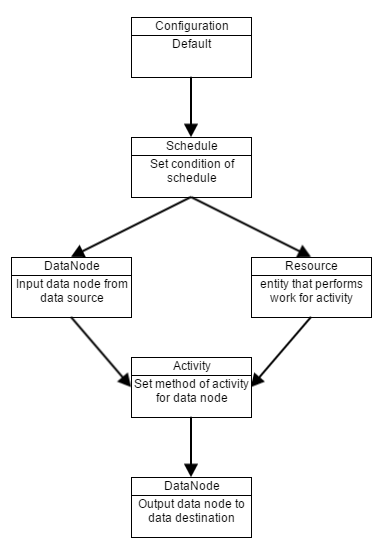
\includegraphics[width=10cm, height=9cm]{data_pipeline.png}
        \centering
        \caption{Complete structure of Data Pipeline}
    \end{figure}
    
	\subsection{Interaction}
	AWS provides management console to create a data pipeline directly. The developer can set the data source and data destination, and then the new data pipeline will automatically make  a connection between these two locations.  
    
\subsection{ Algorithm}
	In this product, the locations are S3 and DynamoDB for data pipeline, thus all of algorithms must be associated to these two services. AWS Data Pipeline supports \textbf{S3DataNode} and \textbf{DynamoDBDataNode}. The  object example of \textbf{S3dataNode} is
	\begin{lstlisting}[caption=S3 Data Node example\cite{z6}]
        {
            "id" : "OutputData",
            "type" : "S3DataNode",
            "schedule" : { "ref" : "CopyPeriod" },
            "filePath" : "s3://myBucket/#{@scheduledStartTime}.csv"
        }
	\end{lstlisting}
	And the object example of \textbf{DynamoDBDataNode} is 
	\begin{lstlisting}[caption=DynamoDB Data Node example\cite{z7}]
        {
            "id" : "MyDynamoDBTable",
            "type" : "DynamoDBDataNode",
            "schedule" : { "ref" : "CopyPeriod" },
            "tableName" : "adEvents",
            "precondition" : { "ref" : "Ready" }
        }
	\end{lstlisting}
	In term of algorithm of activity, AWS Data pipeline provides several general activities to accommodate common scenarios. These activities include \textbf{CopyActivity}, \textbf{HiveActivity}, \textbf{PigActivity}, etc.\\ 
    
    \noindent Resource is used to make these activities work on data node. The AWS Data Pipeline supports two kinds of resources: EC2 and EMR. The concept of \textbf{Ec2Resource} is to use EC2 instance to perform the activity but \textbf{EmrCluster} is to use EMR cluster to perform the activity. 

